\documentclass[aspectratio=169]{beamer}
\setbeamertemplate{footline}[frame number]
%\documentclass[aspectratio=169,notes=only]{beamer}
\usepackage{multicol}
\usepackage{wrapfig}
\usepackage{algorithmicx}
\usepackage{algpseudocode}
\usepackage{graphicx}
%\usepackage{subcaption} % cannot be used

\usepackage[english]{layout}
\usepackage[utf8]{inputenc}
\usepackage[english]{babel}
\usepackage[T1]{fontenc}
\usepackage{amsmath, soul, color, multicol, type1cm, verbatim, latexsym, dsfont, float, listings,alltt,tikz, lmodern, textcomp}
\usepackage[official]{eurosym}
\usepackage[export]{adjustbox}
\usepackage[caption = false]{subfig}
%\usepackage{beamerthemesplit}
%\usetheme{Frankfurt}
\usecolortheme{lily}
%\usefonttheme{structuresmallcapsserif}
\usefonttheme{professionalfonts}
\setbeamercovered{transparent}

\newcommand{\pluseq}{\mathrel{{+}{=}}}

%NeSI Colors <-------------------------------------------------------------------------------------
\usecolortheme{lily}
\usecolortheme[RGB={47, 68, 71}]{structure} 
\definecolor{nesidark}{HTML}{2F4447}
\definecolor{nesilight}{HTML}{CED9DF}
\definecolor{nesigrey}{gray}{0.7}
\definecolor{nesilightgrey}{gray}{0.98}
\definecolor{nesidarkgrey}{gray}{0.3}
\definecolor{nesiblue}{HTML}{2B9FC2}
\setbeamercolor{block title}{fg=black,bg=nesigrey}
\setbeamercolor{block body}{bg=nesilightgrey,fg=nesidarkgrey}
\setbeamercolor{block body alerted}{bg=white,fg=black}
\setbeamercolor{alerted text}{bg=white,fg=black}
\addtobeamertemplate{frametitle}{\vskip+1.2ex}{}
%NeSI Custom Code Hightlight <---------------------------------------------------------------------------------------
\lstdefinestyle{customcode}{
  belowcaptionskip=1\baselineskip,
  breaklines=true,
  xleftmargin=\parindent,
  showstringspaces=false,
  basicstyle=\ttfamily,
  keywordstyle=\bfseries\color{green!40!black},
  commentstyle=\itshape\color{purple!40!black},
  identifierstyle=\color{blue},
  stringstyle=\color{orange},
}
%NeSI Title <---------------------------------------------------------------------------------------
\setbeamerfont{title}{size=\huge}
\frenchspacing
\hyphenation{NeSI}
%NeSI Template parameters <-------------------------------------------------------------------------
\setbeamertemplate{blocks}[default]
\useinnertheme{circles}
\setbeamertemplate{title page}[default][center,rounded=false,shadow=false]
\newcommand\BackgroundPicture[1]{%
\setbeamertemplate{background}{%
\parbox[c][\paperheight]{\paperwidth}{%
\vfill \hfill \includegraphics[height=\paperheight]{#1}
\hfill \vfill
}}}

%\pagenumbering{arabic}

%Content Starts Here <-------------------------------------------------------------------------------
\title{\LARGE{Mimetic postprocessing for LFRic\\}}
%\subtitle{Computational Science team}
\author{\\
Alexander Pletzer (NeSI/NIWA), Wolfgang Hayek (NIWA/NeSI) and Jorge Bornemann (NIWA) \\
(alexander.pletzer@nesi.org.nz) \\
Sam Adams, Mike Hobson  and Nigel Wood (UK MetOffice) \\
 LFRic Melbourne Workshop 20-23 Feb 2018  }
\date{}

\begin{document}
\BackgroundPicture{NeSI/title.png}
\begin{frame}[plain]
  \vspace{+1.0cm}
  \titlepage
\end{frame}

% This will generate the outline. If you have several topics, uncomment the multicols 
\BackgroundPicture{NeSI/blank-01.png}

%%%%%%%%%%%%%%%%%%%%%%%%%%%%%%%%%%%%%%%%%%%%%%%%%%%%%%%%%%%%%%%%%%%%%%%%%%%%%%%%%%%%%%%%%%%%%%%
%%%%%%%%%%%%%%%%%%%%%%%%%%%%%%%%%%%%%%%% Some Examples %%%%%%%%%%%%%%%%%%%%%%%%%%%%%%%%%%%%%%%%
%%%%%%%%%%%%%%%%%%%%%%%%%%%%%%%%%%%%%%%%%%%%%%%%%%%%%%%%%%%%%%%%%%%%%%%%%%%%%%%%%%%%%%%%%%%%%%%
% List with bullets (itemize) <---
% The [<+-| alert@+>] will create a new slide for each element with highlighting 

\BackgroundPicture{NeSI/divider-01.png}
\begin{frame}[fragile]{}
  \begin{center}
    \Huge{\textbf{Why we need to worry about pre-/post-processing}}
  \end{center}
\end{frame}
\BackgroundPicture{NeSI/blank-01.png}

\begin{frame}[t]
  \frametitle{Not business as usual}
    \begin{block}{}
      \begin{enumerate}%[<+-| alert@+>]
	  \item GungHo's horizontal grid is {\color{red} unstructured}. Iris handles structured grids only.
      \item Grid cells are {\color{red} non-orthogonal}. Watch out for code that implicitly assumes orthogonality.
      \item Fields are on nodes, {\color{red} edges, faces} and cells (mixed finite elements) $\rightarrow$ UGRID fields.
      \item Support for {\color{red} high order} finite elements. There is no standard! 
      \end{enumerate}
  \end{block}
\begin{figure}[!htb]
\centering
\begin{minipage}{0.4\textwidth}
  \centering
  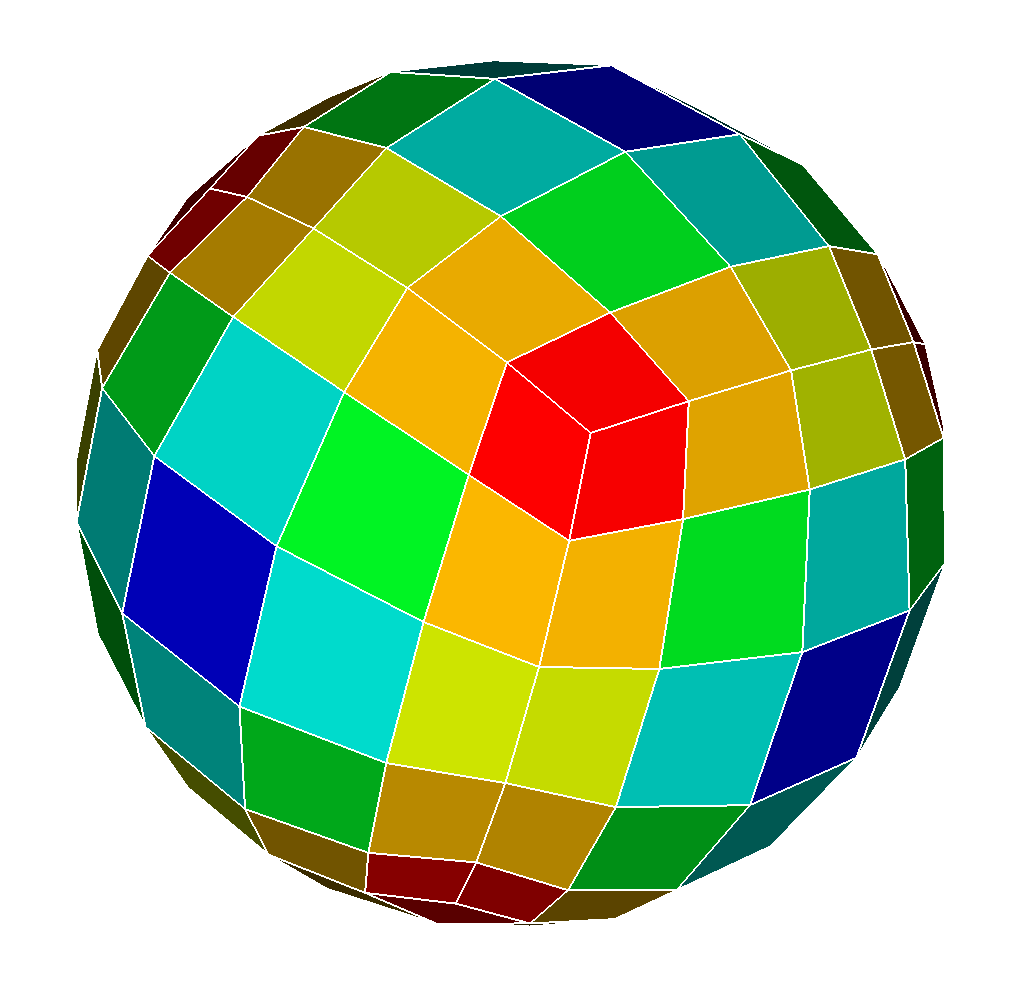
\includegraphics[width=0.45 \linewidth]{cubedSphere.png}
  %\caption{Cubed-sphere}
\end{minipage}%
\begin{minipage}{.5\textwidth}
  \centering
  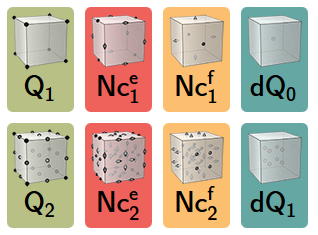
\includegraphics[width=0.45 \linewidth]{nodeEdgeFaceCellElements.png}
  %\caption{Mixed finite elements}
\end{minipage}
\end{figure}
\end{frame}

\begin{frame}[t]
  \frametitle{Mimetic discretization impacts many areas of pre- and post-processing}
    \begin{block}{}
      \begin{itemize}%[<+-| alert@+>]
	  \item Regridding/remapping
      \begin{itemize}
        \item Scientists want to see results in lat-lon space
      \end{itemize}
      \item Visualization
      \begin{itemize}
        \item E.g. streamlines need to compute the velocity 
      \end{itemize}
      \item Transport of tracers
      \begin{itemize}
        \item Langragian formulation $\equiv$ interpolate field at previous position 
      \end{itemize}
      \item Computation of fluxes
      \end{itemize}
    All the above need {\color{red} interpolation} in one form  or another
  \end{block}
\end{frame}

\begin{frame}[t]
  \frametitle{The price of not doing it right}
    \begin{block}{}
      \begin{itemize}%[<+-| alert@+>]
	  \item Regridding/remapping: {\color{red} Cannot compare models}, cannot interface, etc.
      \item Visualization: {\color{red} Cannot debug}, community cannot see the benefits of the GungHo approach
      \item Transport of tracers: Lack of {\color{red} conservation}
      \item Computation of fluxes: {\color{red} Spurious inaccuracy} 
      \end{itemize}
  \end{block}
\end{frame}

\begin{frame}[t]
  \frametitle{Example 1: Getting fluxes right}
  \begin{block}{}
   Using $W_1$ finite elements as interpolating functions returns the correct flux whilst a nodal interpolation an error dependent on the grid resolution and the number of segments.
  \end{block}
  
\begin{figure}[!htb]
\centering
\begin{minipage}{.49\textwidth}
  \centering
  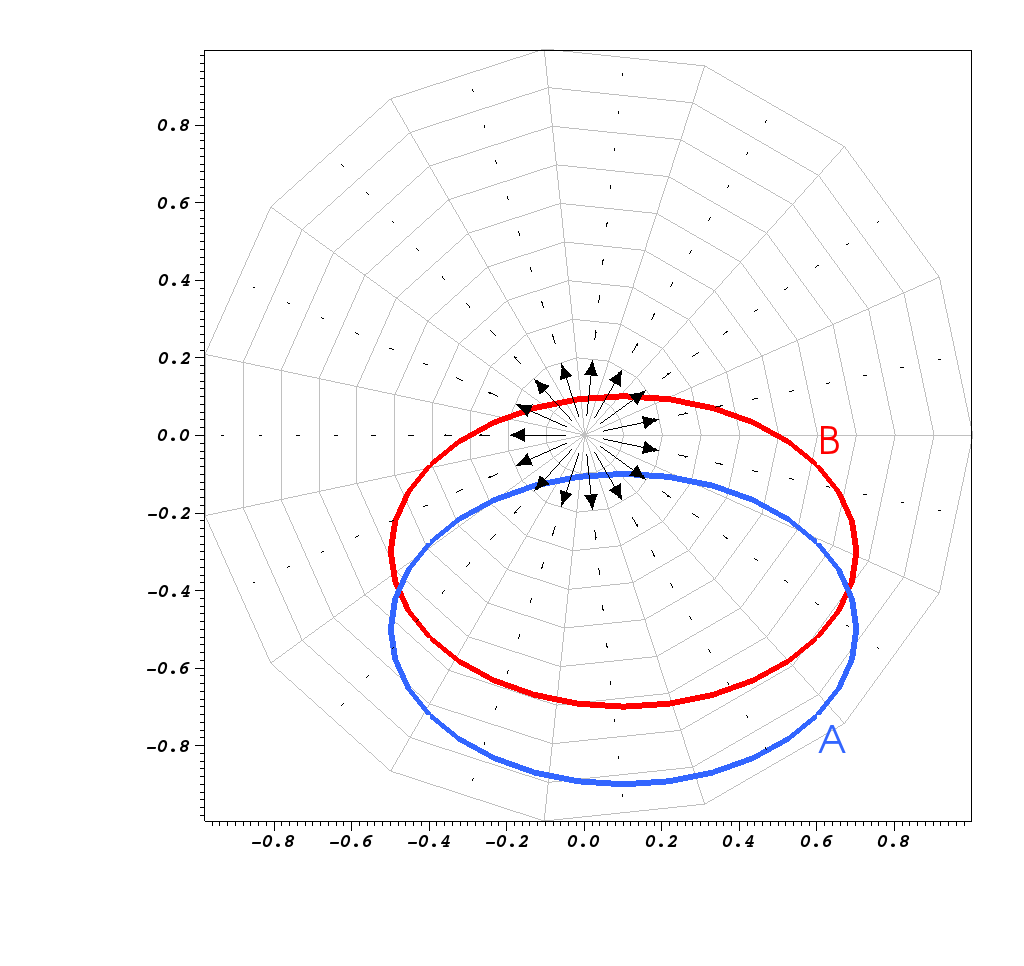
\includegraphics[width=.7\linewidth]{polar.png}
  %\caption{Radial field}
\end{minipage}%
\begin{minipage}{.49\textwidth}
  \centering
  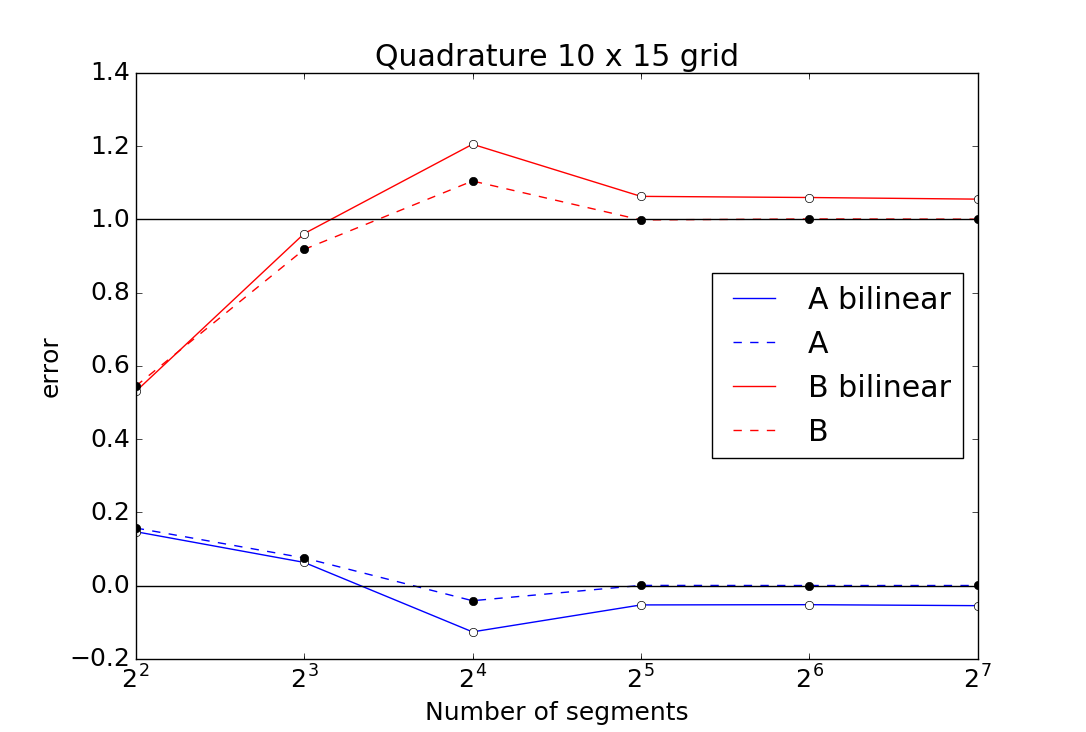
\includegraphics[width=.8\linewidth]{case2ErrorPlotAB.png}
  %\caption{Flux estimate}
\end{minipage}
\end{figure}
\end{frame}

\begin{frame}[t]
  \frametitle{Example 2: transport (advection) of fields}
  \begin{block}{$\partial_t + \mathcal{L}_v$ takes many forms but all these cases can be handled by the same interpolation procedure}
  \begin{itemize}
    \item $\partial_t + v \cdot \nabla \star$ for nodal fields
    \item $\partial_t + (\nabla \times \star) \times v + \nabla (v \cdot \star)$ for edge fields
    \item $\partial_t + \nabla \times (\star \times v) + \nabla \cdot (v \cdot \star)$ for face fields
    \item $\partial_t + \nabla \cdot (v \star)$ for cell fields
    \end{itemize}
  \end{block}
  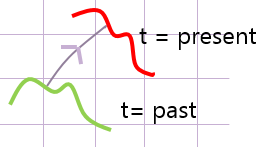
\includegraphics[width=0.3\linewidth]{LieDerivative.png}
\end{frame}

\BackgroundPicture{NeSI/divider-02.png}
\begin{frame}[fragile]{}
  \begin{center}
    \Huge{\textbf{Results}}
  \end{center}
\end{frame}
\BackgroundPicture{NeSI/blank-01.png}

\begin{frame}[t]
  \frametitle{Comparing software for locating a cell}
  \begin{block}{All interpolation methods need to quickly locate cell containing a point}
  \begin{itemize}
    \item findCellVtk: VTK method vtkUnstructured 
    \item findcellEsmf: ESMF software
    \item findCellVtkCellLocator: octree based search. {\color{red} Search time is nearly independent of grid size!}. Average number of cells per bucket is 100.
  \end{itemize}
  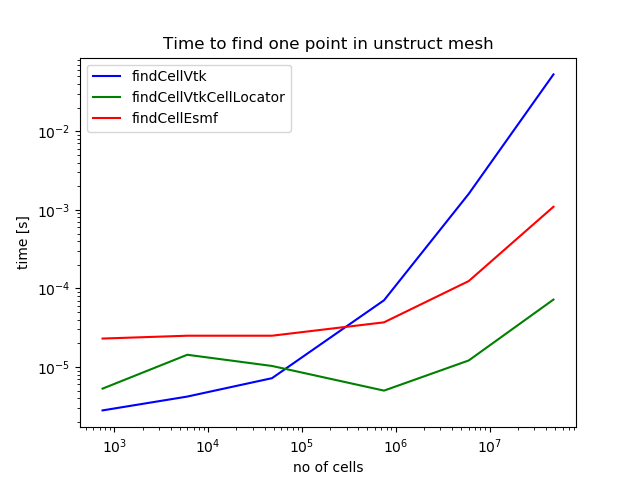
\includegraphics[width=.4\linewidth]{kupe.png}
  \end{block}
\end{frame}

\begin{frame}[t]
  \frametitle{Proposed approach works on the cubed-sphere}
  \begin{block}{}
   \begin{itemize}
   \item Test $v = \nabla \psi \times \nabla r$; $\psi:$ analytic stream function of lat-lon
   \item Flux only depends on start/end points. Zero error if start/end points fall on nodes
   \item Some cells have 120 deg angle between edges
   \end{itemize}
  \end{block}
  
  \begin{tabular}{lr}
  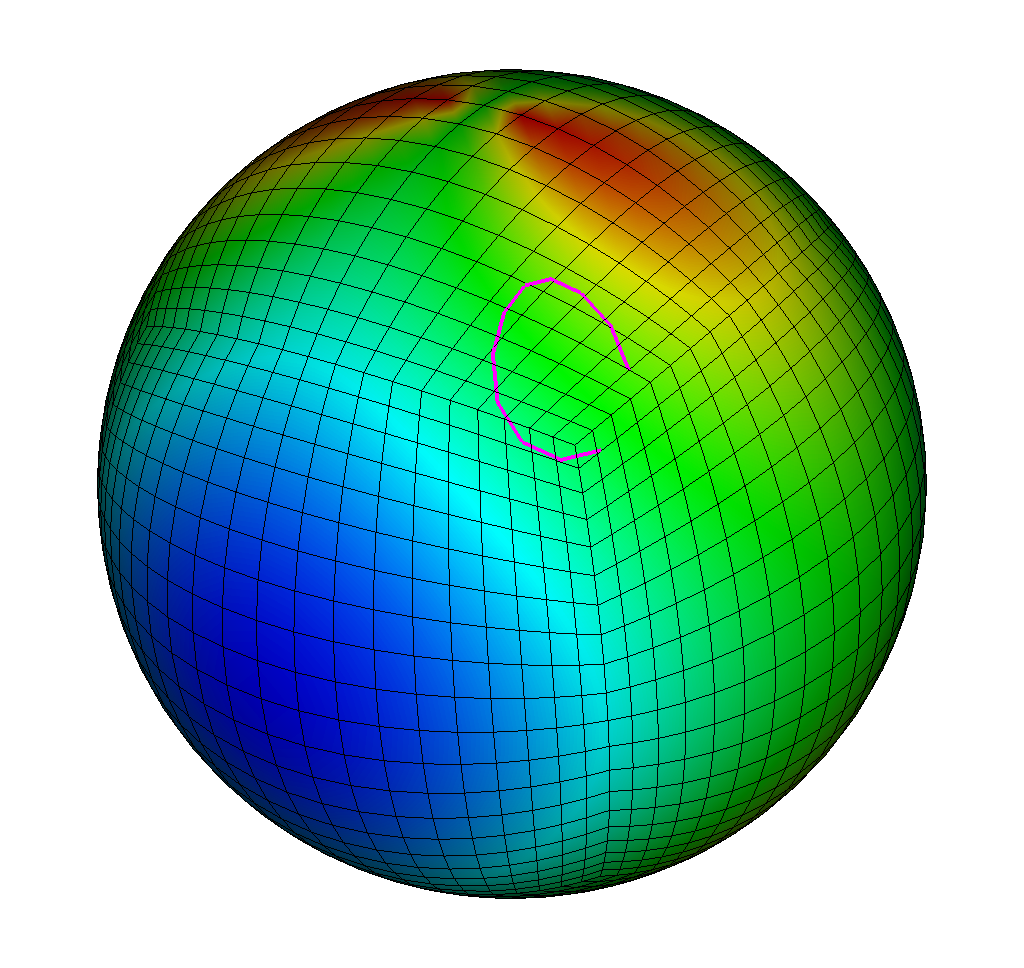
\includegraphics[width=30mm]{fluxOnCubedSphere.png} & 
  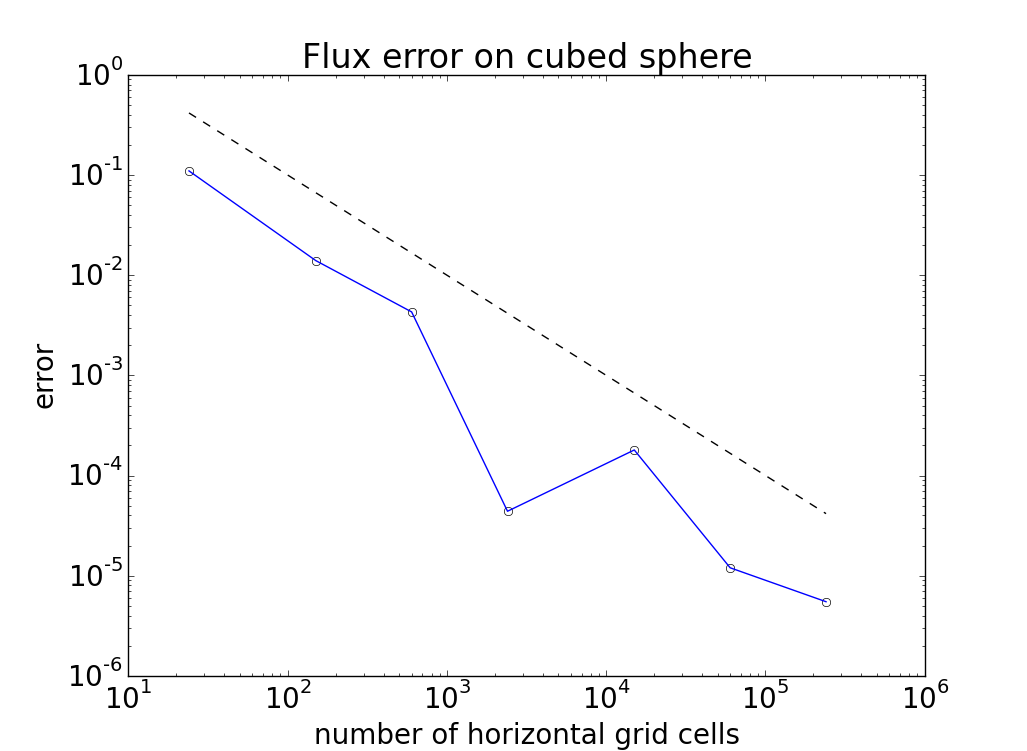
\includegraphics[width=50mm]{cubedSphereFluxError.png} \\
  {Integration path/surface} & {Error is $\sim h^2$} 
  \end{tabular}
\end{frame}

\begin{frame}[t]
  \frametitle{Problem of dateline when using lat-lon coordinates so ended up using Cartesian coordinates}
  \begin{block}{}
   \begin{itemize}
   \item Dateline cannot cross cells
   \item Jagged dateline
   \item Cell at the pole has a cut
   \end{itemize}
  \end{block}
  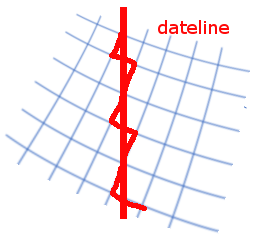
\includegraphics[width=.3\linewidth]{datelineProblem.png}
\end{frame}

\BackgroundPicture{NeSI/divider-04.png}
\begin{frame}[fragile]{}
  \begin{center}
    \Huge{\textbf{Recommended work plan}}
  \end{center}
\end{frame}
\BackgroundPicture{NeSI/blank-01.png}


\begin{frame}[t]
  \frametitle{Step 1: develop a standalone mini-app that takes a collection of points and returns cells and barycentric coordinates for each cell}
    \begin{block}{}
      \begin{itemize}%[<+-| alert@+>]
	  \item Necessary step for interpolation
      \item The only step need to do nodal interpolation
      \item Can use off the shelf software (e.g. VTK) 
      \item Does not depend much on other developments (can proceed in parallel)
      \item Could work with scientist who needs the work
    \end{itemize}
  \end{block}
\end{frame}

\begin{frame}[t]
  \frametitle{Step 2: compute the collision of source and target grids}
    \begin{block}{}
      \begin{itemize}%[<+-| alert@+>]
	  \item Requires step 1 to be completed
      \item Result is a map of target elements $\rightarrow$ set of source grid elements and parametric coords
      \item Custom code (?), API (?) 
    \end{itemize}
  \end{block}
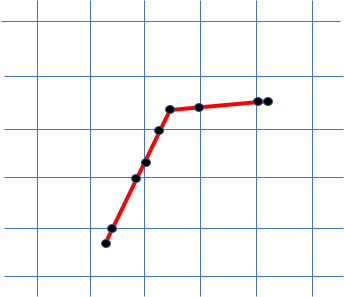
\includegraphics[width=.3\linewidth]{interpStep3.png}\end{frame}

\begin{frame}[t]
  \frametitle{Step 3: evaluate the interpolation weights/integrals }
    \begin{block}{}
      \begin{itemize}%[<+-| alert@+>]
	  \item Requires step 2 to be completed
      \item Fairly straightforward but laborious for high order finite elements
      \item Exact!
    \end{itemize}
  \end{block}
  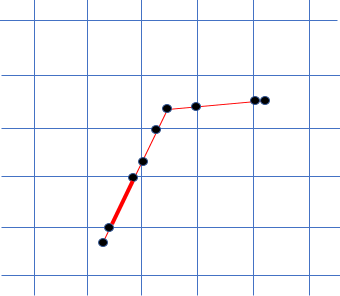
\includegraphics[width=.3\linewidth]{interpStep4.png}
\end{frame}


% End <-----------------------------------------------------------------------------------------
\BackgroundPicture{NeSI/blank-02.png}
\begin{frame}[plain]
  \begin{center}
  Goal is to apply the rigour of dynamical cores to pre- and post-processing tools. Overtime we expect the distinction between dynamical core
  and pre-/post-processing to diminish.
  \\
  
    \vspace*{+2cm}
    {\Huge Thank You}\\
    \vspace*{+1cm}
    
\includegraphics[width=100pt]{NeSI/nesi_logo.png}
  \end{center}
\end{frame}

\end{document}
